\DiaryEntry{Convolutional Codes, Error Analysis}{2019-04-08}{Coding}

The coded bits are transmitted via a channel which introduces bit errors. These bit errors can cause the Viterbi algorithm to select a different path through the trellis as the path caused by the information bits. This different path can then cause a different information bit sequence and thereby cause (information) bit errors.

The error analysis is simplified by the fact that convolutional codes are linear codes; i.e. the sum of two code sequences is another code sequence. Therefore it is sufficient to consider transmission of the all-zero information bit sequence and consider its bit errors only. That is, we consider the all-zero path through the trellis; code bit errors then cause deviations from this path and these may lead to information bit erros.

\subsection{Path Enumeration}

It is necessary to enumerate the trellis paths; i.e. collect the information about how many information bits equal one cause a certain path and how many code bits equal one this path has. To this end we split the all-zero state of the trellis into two and consider the "transfer function" between these two states. This is shown for the $(5,7)$ code in the Figure below.

Splitting the trellis in such a way yields the following Figure.

\vspace*{7mm}

\begin{tikzpicture}

  \SetUpEdge[lw=1.5pt, color=blue]

  \GraphInit[vstyle=Normal]
  \SetGraphUnit{4}
  \tikzset{VertexStyle/.append style={fill}}

  \Vertex[x=0, y=0]{00[start]}
  \Vertex[x=4, y=0]{10}
  \Vertex[x=8, y=0]{01}
  \Vertex[x=6, y=-5]{11}
  \Vertex[x=12, y=0]{00[stop]}
  
  \tikzset{EdgeStyle/.style={->}}
  
  \Edge[label=$1/11$](00[start])(10)
  \Edge[label=$0/01$](10)(01)
  \Edge[label=$0/11$](01)(00[stop])
  \Edge[label=$1/10$](10)(11)
  \Edge[label=$0/10$](11)(01)

  \Loop[label=$1/01$, dir=SO, labelstyle={above},style={blue, very thick}](11)

  \tikzset{EdgeStyle/.append style = {bend right}}
  \Edge[label=$1/00$](01)(10)

\end{tikzpicture}

\paragraph{Rules}

To calculate the transfer function, we have the following rules

\begin{itemize}

\item Blocks in series multiply their transfer functions.

\item Blocks in parallel add the transfer functions.

\item Blocks with feedback loop use the rule, "forward amplification divided by one minus loop gain".

\end{itemize}

We want a transfer function which connects the information bit weight with the code bits weight. To this end, we assign every edge in the graph a polynom of the form $N^a D^b$, where $N, D$ are dummy variables, $a$ is the information bit weight, and $b$ is the corresponding code bit weight.

\vspace*{7mm}

\begin{tikzpicture}

  \SetUpEdge[lw=1.5pt, color=blue]

  \GraphInit[vstyle=Normal]
  \SetGraphUnit{4}
  \tikzset{VertexStyle/.append style={fill}}

  \Vertex[x=0, y=0]{00[start]}
  \Vertex[x=4, y=0]{10}
  \Vertex[x=8, y=0]{01}
  \Vertex[x=6, y=-5]{11}
  \Vertex[x=12, y=0]{00[stop]}
  
  \tikzset{EdgeStyle/.style={->}}
  
  \Edge[label=$ND^2$](00[start])(10)
  \Edge[label=$D$](10)(01)
  \Edge[label=$D^2$](01)(00[stop])
  \Edge[label=$ND$](10)(11)
  \Edge[label=$D$](11)(01)

  \Loop[label=$ND$, dir=SO, labelstyle={above},style={blue, very thick}](11)

  \tikzset{EdgeStyle/.append style = {bend right}}
  \Edge[label=$N$](01)(10)

\end{tikzpicture}

In the following we calculate the transfer function of the whole trellis in a step-wise (bottom-up) maner.

We first calcuate the transfer function of the loop around state $11$ (which is $\frac{1}{1-ND}$) and combine it with the transfer functions of the series $ND$ and $D$. This yields the following Figure.

\vspace*{7mm}

\begin{tikzpicture}

  \SetUpEdge[lw=1.5pt, color=blue]

  \GraphInit[vstyle=Normal]
  \SetGraphUnit{4}
  \tikzset{VertexStyle/.append style={fill}}

  \Vertex[x=0, y=0]{00[start]}
  \Vertex[x=4, y=0]{10}
  \Vertex[x=8, y=0]{01}
  \Vertex[x=12, y=0]{00[stop]}
  
  \tikzset{EdgeStyle/.style={->}}
  
  \Edge[label=$ND^2$](00[start])(10)
  \Edge[label=$D$](10)(01)
  \Edge[label=$D^2$](01)(00[stop])
  
  \tikzset{EdgeStyle/.append style = {bend right}}
  \Edge[label=$N$](01)(10)

  \tikzset{EdgeStyle/.append style = {bend right}}
  \Edge[label=$\frac{ND^2}{1-ND}$](10)(01)

\end{tikzpicture}

Combining the two transfer functions from states $10$ to $01$ yields

\bee
D + \frac{ND^2}{1-ND} = \frac{D - ND^2 + ND^2}{1-ND} = \frac{D}{1-ND}
\eee

which yields the following Figure.

\vspace*{7mm}

\begin{tikzpicture}

  \SetUpEdge[lw=1.5pt, color=blue]

  \GraphInit[vstyle=Normal]
  \SetGraphUnit{4}
  \tikzset{VertexStyle/.append style={fill}}

  \Vertex[x=0, y=0]{00[start]}
  \Vertex[x=4, y=0]{10}
  \Vertex[x=8, y=0]{01}
  \Vertex[x=12, y=0]{00[stop]}
  
  \tikzset{EdgeStyle/.style={->}}
  
  \Edge[label=$ND^2$](00[start])(10)
  \Edge[label=$D^2$](01)(00[stop])
  
  \tikzset{EdgeStyle/.append style = {bend right}}
  \Edge[label=$N$](01)(10)

  \tikzset{EdgeStyle/.append style = {bend right}}
  \Edge[label=$\frac{D}{1-ND}$](10)(01)

\end{tikzpicture}

We finally calculate the transfer function of the feedback loop,

\bee
\frac{ \frac{D}{1-ND} }{1 - \frac{ND}{1-ND}} = \frac{ \frac{D}{1-ND} }{ \frac{1-2ND}{1-ND} } = \frac{D}{1-2ND}
\eee

 and arrive at the following Figure.

\vspace*{7mm}

\begin{tikzpicture}

  \SetUpEdge[lw=1.5pt, color=blue]

  \GraphInit[vstyle=Normal]
  \SetGraphUnit{4}
  \tikzset{VertexStyle/.append style={fill}}

  \Vertex[x=0, y=0]{00[start]}
  \Vertex[x=4, y=0]{10}
  \Vertex[x=8, y=0]{01}
  \Vertex[x=12, y=0]{00[stop]}
  
  \tikzset{EdgeStyle/.style={->}}
  
  \Edge[label=$ND^2$](00[start])(10)
  \Edge[label=$D^2$](01)(00[stop])
  \Edge[label=$\frac{D}{1-2ND}$](10)(01)

\end{tikzpicture}

This yields a transfer function of the complete trellis as

\bee
H(N,L) = \frac{ND^5}{1-2ND} = ND^5 + 2N^2D^6 + 4N^3D7 + \cdots
\eee

where we have made a series expansion as well. The series expansion provides the following facts

\begin{itemize}

\item There is one path with code bit weight $5$ and information bit weight $1$. This corresponds to the following state sequence through the trellis: $00-10-01-00$.

\item  There are two paths with code bit weight $6$ and information bit weight $2$. These correspond to the state sequences $00-10-11-01-00$ and $00-10-01-10-01-00$, respectively.

\end{itemize}

\subsection{Error Analysis}

Let $\mathcal{P}_j$ denote the set of all error paths that diverge from node $j$ of the all-zero path in the trelis and remerge later. Let $p_{i,j}$ be one such path and let $\Delta M(p_{i,j})$ be the difference between the metric accumulated along this path and the all-zero path. An error event (at node $j$) occurs due to path $p_{i,j}$, if $\Delta M(p_{i,j}) < 0$. Denoting with $P_e(j)$ the probability of an error event at node $j$, we have

\bee
P_e(j) \leq Pr \left[ \cup_i \{ \Delta M(p_{i,j}) < 0 \} \right]
\eee

The paths $p_{i,j}$ are not disjoint but may share branches so the events in above expression are not disjoint. This makes an exact calculation very difficult and we consider a union bound instead,

\bee
P_e(j) \leq \sum_i Pr(\Delta M(p_{i,j}) < 0)
\eee

Each term in this summation is a pairwise event between the paths $p_{i,j}$ and the all-zero path. For a memoryless channel, $\Delta M(p_{i,j})$ depends only on those branches for which $p_{i,j}$ is nonzero. Let $d$ be the Hamming weight of $p_{i,j}$, let$a(d)$ be the number of paths at distance $d$ away from the all-zero path, and let $P_d$ be the probability of the event that this path has a lower metric than the all-zero path. The node error probability can then be rewritten as

\bee
P_e(j) \leq \sum_{d=d_{free}}^\infty a(d) P_d
\eee

Wew ill show below that $P_d < Z^d$ for some function $Z$ depending on the channel. With this, we can write

\bee
P_e(j) \leq \sum_{d=d_{free}}^\infty a(d) Z^d = T(D)|_{D=Z}
\eee

where we have used the path enumerator $T(D) = \sum_{d=d_{free}}^\infty a(d) D^d$. The above is a bound on the node error probability from which we can obtain a bound on the bit error probability by enumerating the number of bits in error for each node error. The derivative

\bee
\frac{\partial}{\partial N} H(D,N)
\eee

brins exponents down as multipliers in each term of the series. The average number of bits in error along a branch of the trellis is

\bee
\frac{\partial}{\partial N} H(D,N)|_{N=1, D=Z}
\eee

For a rate $R=k/n$ code, each branch corresponds to $k$ information bits, so that

\bee
P_b < \frac{1}{k} \frac{\partial}{\partial N} H(D,N)|_{N=1, D=Z}
\eee

If we consider only the first term in the series (which is a good approximation for large SNR values), we have

\bee
\frac{\partial}{\partial N} H(D,N)|_{N=1} = D^{d_{free}} (n_1 + n_2 + \cdots ) + D^{d_{free}+1} (\cdots) + \cdots
\eee

and the number $b_{d_{free}} = n_1 + n_2 + \cdots$ is the number of non-zero information bits associated with code words of weight $d_{free}$.

In our running example of $H(N,L) = \frac{ND^5}{1-2ND} = ND^5 + 2N^2D^6 + 4N^3D7 + \cdots$, we have $d_{free} = 5$ and there are $b_{d_{free}} = 1$ information bits associated with this code word.

This allows for the final bound

\bee
P_b > \frac{1}{k} b_{d_{free}} D^{d_{free}}
\eee



\subsection{A bound on $P_d$ for the AWGN channel}

The error detection probability on the AWGN channel is given by

\bee
P_d = Q \left( \sqrt{\frac{2dE_c}{N_0} } \right)
\eee

Several bounds later, we arrive at

\bee
P_b > \frac{1}{k} b_{d_{free}} Q \left( \sqrt{\frac{2 d_{free} E_c}{N_0} } \right) = \frac{1}{2k} b_{d_{free}} \erf \left( \sqrt{\frac{d_{free} E_c}{N_0} } \right)
\eee

For the running example of the $(5,7)$ code, $k=2, d_{free} = 5$ and $b_{d_{free}} = 1$.



%%% Local Variables:
%%% mode: latex
%%% TeX-master: "journal"
%%% End:
